% -----------------------------------------------------------------------
% CCN 2026 - Camera-Ready Extended Abstract
% -----------------------------------------------------------------------
\documentclass[extended-abstract]{ccn}

\addbibresource{ccn_references.bib}

\emergencystretch=3em


\title{Fine-Grained Emotion Structure in the Brain-Aligned Subspace of a Self-Supervised Video Model}

\author{%
  Seokjin Moon\affmark{1} \And
  Taeyang Lee\affmark{2} \And
  Jiook Cha\affmark{1,2}%
}
\affiliation{1}{Department of Brain and Cognitive Sciences, Seoul National University}
\affiliation{2}{Department of Psychology, Seoul National University}
\emails{moon97322@snu.ac.kr, rlaxodid5539@snu.ac.kr, connectome@snu.ac.kr}


\begin{document}

\maketitle

\begin{abstract}
  Do the brain and self-supervised video models share a common structure for representing emotion?
  Prior work showed that neural responses to emotional videos are better explained by fine-grained emotion categories than by affective dimensions (valence, arousal).
  We ask whether this categorical structure extends to the subspace shared between the human brain and a video foundation model trained without emotion labels.
  By aligning neural representations from Brain-JEPA with embeddings from V-JEPA2, we identify a compact brain-aligned subspace restricted to only three of the leading principal components of a 1{,}408-dimensional embedding.
  This shared subspace shows stronger geometric alignment with discrete emotion categories than with affective dimensions, with a larger category-over-valence-arousal advantage than in the full video model space and stable across all individual subjects.
  These findings suggest that visually shared brain-model representations preferentially preserve category-like emotion structure, whereas dimensional affective information may rely more strongly on brain components not captured by this visual model-aligned subspace.
\end{abstract}

\textbf{Keywords:} emotion representation, fMRI, video foundation model, self-supervised learning, brain-aligned subspace

\section{Introduction}

A central question in affective neuroscience is whether the brain organizes emotional experience along continuous affective dimensions such as valence and arousal \citep{Russell1980}, or as a high-dimensional space of fine-grained categories \citep{CowenKeltner2017}.
\citet{Horikawa2020} showed that whole-brain fMRI responses to over 2{,}000 emotional videos are better predicted by fine-grained categories than by affective dimensions.
Artificial neural networks can also predict emotional responses to visual stimuli \citep{Kragel2019,Conwell2025}, but prior work has relied on supervised models or behavioral rather than direct neural measurements.
Self-supervised video foundation models learn structured visual representations from large-scale video without semantic or affective supervision.
Here we examine the affective geometry of the subspace shared between such models and the brain, aligning Brain-JEPA \citep{Dong2024} representations with embeddings from V-JEPA2 \citep{Assran2025}, a self-supervised video model trained on over one million hours of video, and find that this brain-aligned subspace of V-JEPA2 is compact and shows stronger geometric alignment with categorical than dimensional emotion structure.

\section{Methods}

We used the fMRI dataset of \citet{Horikawa2020} (5 subjects, 2{,}196 stimulus presentations of emotionally evocative video clips) with crowd-sourced scores for 34 emotion categories and 14 affective dimensions \citep{CowenKeltner2017}.
For each subject and each video, we extracted a video-level Brain-JEPA embedding from the stimulus-evoked fMRI response, and averaged these across the five subjects to obtain a subject-invariant brain embedding.
V-JEPA2 video embeddings were obtained by uniformly sampling 16 frames and mean-pooling the final hidden state ($2196 \times 1408$).

We decomposed V-JEPA2 into 100 principal components (PCs) and predicted each from Brain-JEPA via 5-fold cross-validated ridge.
PCs surviving permutation-based FDR ($q<0.05$, $n=1{,}000$) were defined as brain-aligned.
From this subspace we decoded 34 emotion categories and, among the 14 affective dimensions, focused on valence and arousal (V-A) as the canonical two-dimensional affective model, using ridge regression with the same 5-fold cross-validation scheme.
We then computed the category/V-A $R^2$ ratio against the same ratio in the full 100-PC space as baseline.
Per-subject stability was tested via one-sided Wilcoxon signed-rank against ratio $\leq 1$.
To test whether categorical alignment was reducible to low-level visual or annotated semantic content, we residualized model embeddings with respect to VGG19 (1{,}000-dim) and human-annotated semantic features (73-dim).
Robustness was further checked with untrained Brain-JEPA, 450-parcel raw BOLD, and in the reverse direction (both sides at 100 PCs).

\section{Results}

Only three of 100 PCs survived FDR correction (PC1 $R^2=0.373$, PC2 $0.075$, PC3 $0.088$), with PC1 stable across all five subjects.
These brain-aligned PCs showed substantially stronger maximum absolute Spearman correlations with emotion categories than brain-unaligned PCs (mean max~$|r|=0.33$ vs.~$0.09$, FDR-corrected), suggesting that the brain-aligned PCs are enriched for affectively relevant variation (Figure~\ref{fig:subspace}).

% ---- FIGURE 1 ----
% Place panel_A_pcscree.png (top) and panel_B_maxr.png (bottom).
\begin{figure}[ht]
  \begin{center}
    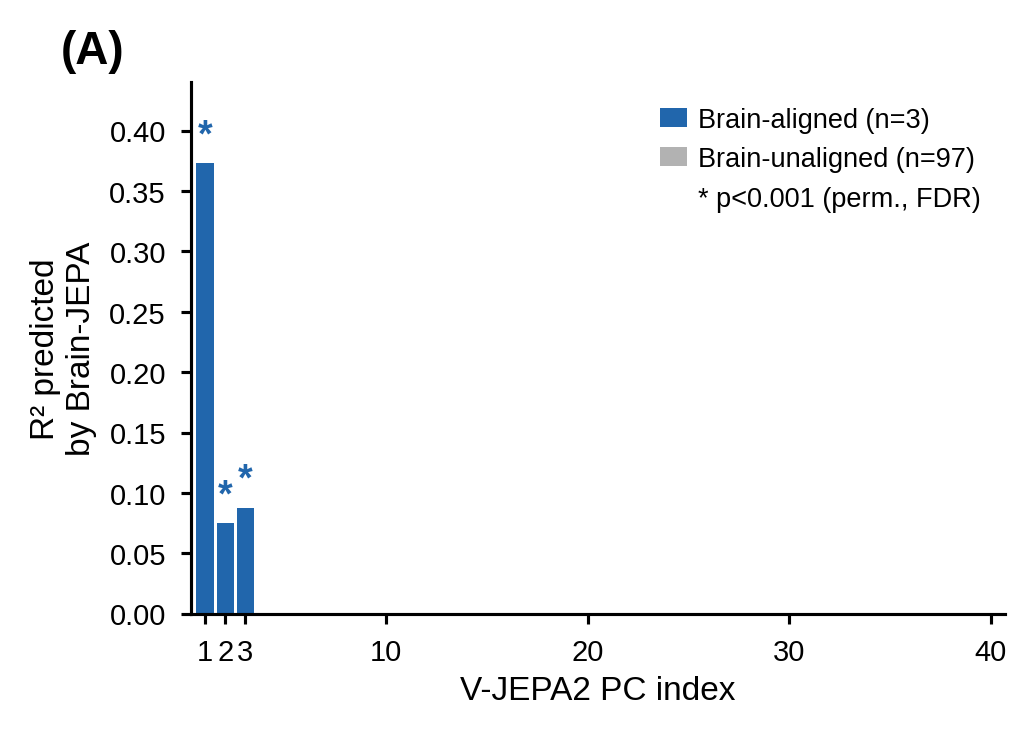
\includegraphics[width=0.8\columnwidth]{panel_A_pcscree.png}\\
    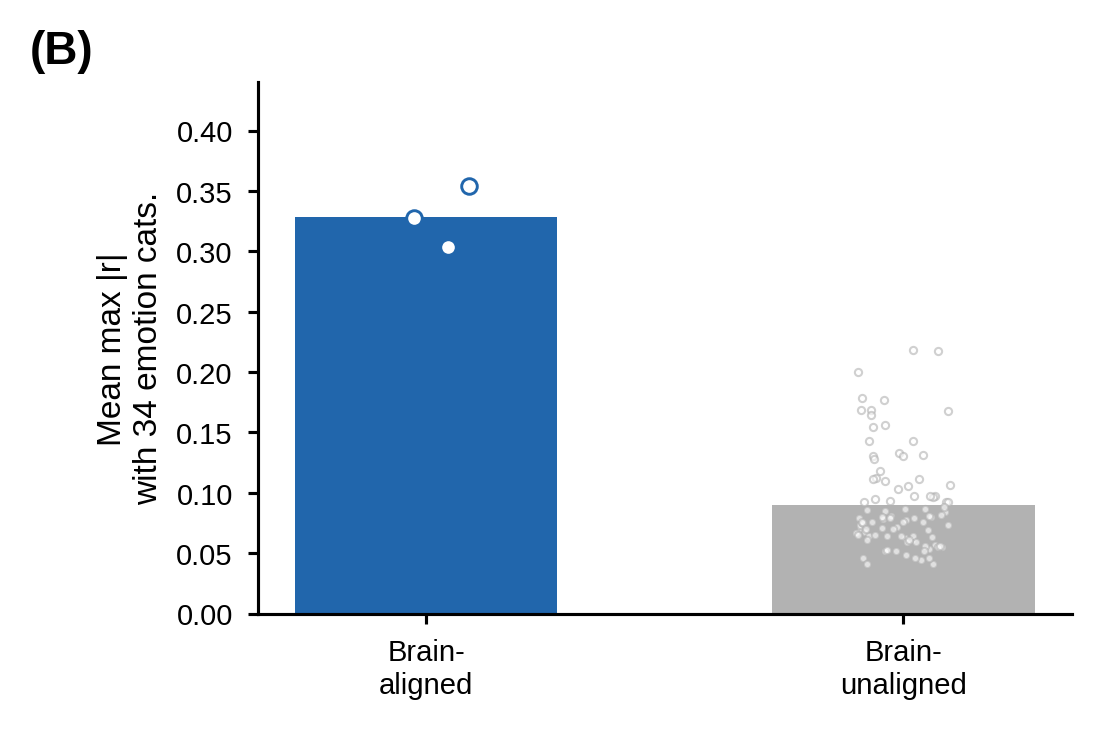
\includegraphics[width=0.8\columnwidth]{panel_B_maxr.png}
  \end{center}
  \caption{Brain-aligned subspace of V-JEPA2.
    (A) $R^2$ predicting each V-JEPA2 PC from Brain-JEPA, with PC1 to PC3 surviving permutation FDR.
    (B) Mean max $|r|$ with 34 emotion categories, brain-aligned vs unaligned PCs.}
  \label{fig:subspace}
\end{figure}

Decoding from this subspace yielded stronger prediction of emotion categories than valence and arousal (mean $R^2 = 0.055$ vs.~$0.038$, $\Delta R^2 = 0.017$, category/V-A ratio $=1.44$), exceeding the full V-JEPA2 100-PC baseline (ratio $=1.26$).
The pattern held across all five subjects (per-subject ratios from 1.96 to 2.65, $p=0.031$).
Partialling out low-level vision and semantic features reduced absolute predictive values, but the categorical advantage of the shared subspace was attenuated rather than eliminated (Figure~\ref{fig:categorical}).

% ---- FIGURE 2 ----
% Place panel_C_decoding.png (top) and panel_D_ratio.png (bottom).
\begin{figure}[ht]
  \begin{center}
    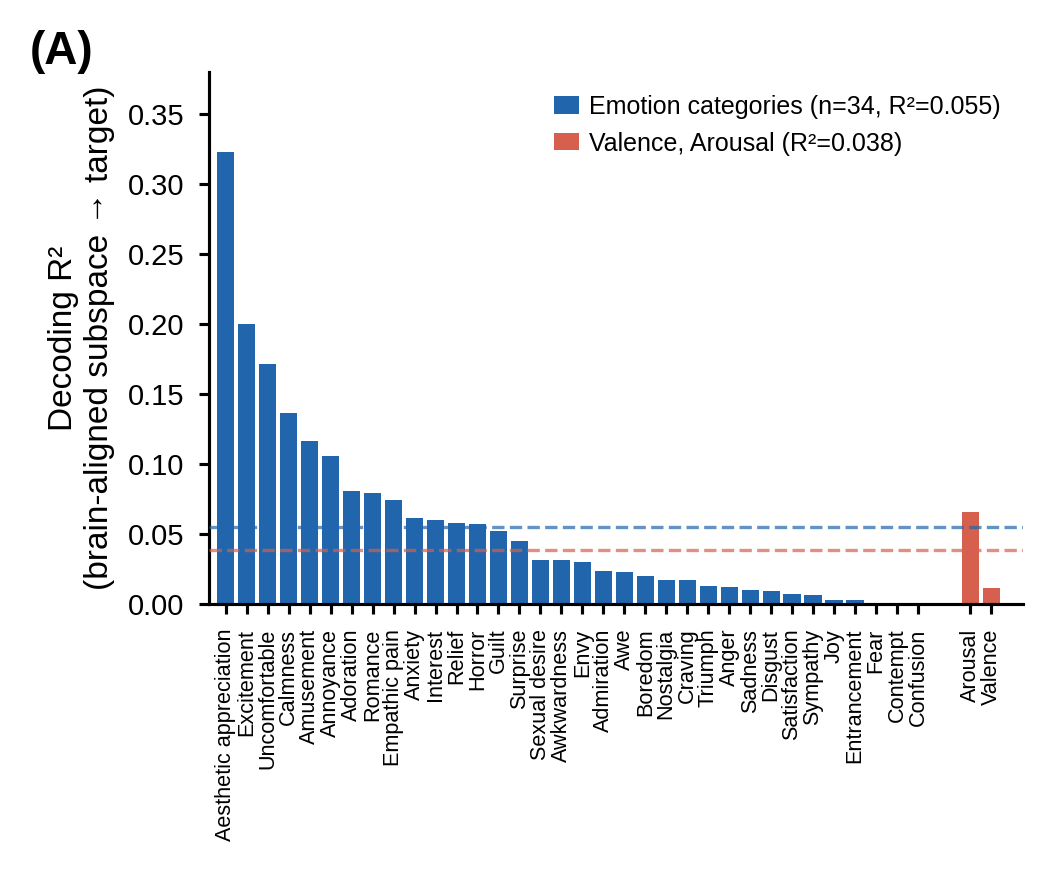
\includegraphics[width=0.8\columnwidth]{panel_C_decoding.png}\\
    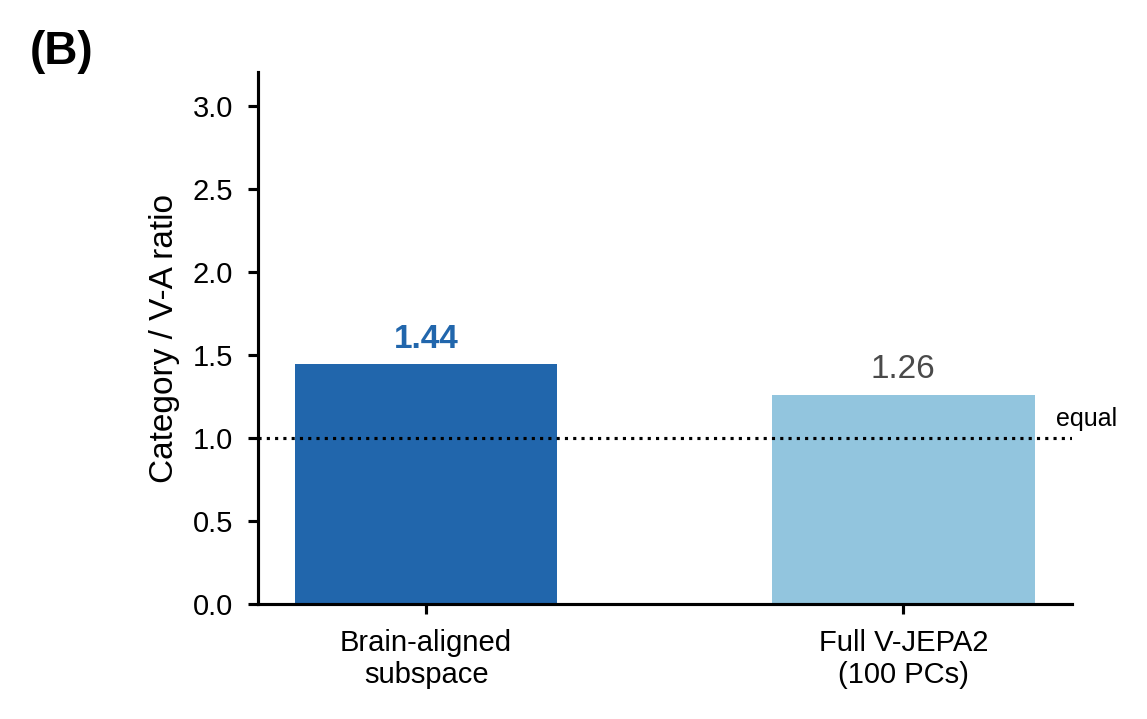
\includegraphics[width=0.8\columnwidth]{panel_D_ratio.png}
  \end{center}
  \caption{Categorical emotion structure of the brain-aligned subspace.
    (A) Decoding $R^2$ across 34 categories from the brain-aligned subspace, with Valence and Arousal in red.
    (B) Category/V-A ratio, brain-aligned subspace vs full V-JEPA2.}
  \label{fig:categorical}
\end{figure}

\section{Discussion}

The representational space shared between a self-supervised video model and the human brain is remarkably compact (3 of 100 PCs, dominated by PC1, $R^2=0.373$).
Inside this subspace the geometry of emotional videos aligns more strongly with discrete categories than with valence and arousal (ratio 1.44 vs.~1.26 in the full V-JEPA2 space, 1.96 to 2.65 per subject, $p=0.031$), paralleling the category-preferential structure reported by Horikawa et al.\ in raw fMRI but in a label-free, self-supervised framing.

The asymmetry persists across alternative brain-side encoders (untrained Brain-JEPA, raw 450-parcel BOLD) and in the reverse direction.
The brain's full space favored dimensional decoding (ratios from 0.60 to 0.76), yet its V-JEPA2-aligned subspace reversed toward a categorical advantage (top-3 ratios from 1.05 to 1.42).
One interpretation, consistent with constructionist accounts, is that visually grounded features contribute more strongly to category-like emotion structure, whereas dimensional affective structure may depend more on non-visual or higher-order brain components.
Future work will extend the analysis to visual-language models such as CLIP \citep{Doerig2025} and decompose the non-visual sources of dimensional structure.

\section*{Acknowledgments}

This work was supported by the National Research Foundation of Korea (NRF) grant funded by the Korea government (MSIT) (No.\ 2021R1C1C1006503, RS-2023-00266787, RS-2023-00265406, RS-2024-00421268, RS-2024-00342301, RS-2024-00435727, RS-2025-25457239, RS-2021-NR061370, NRF-2021M3E5D2A01022515, and NRF-2021S1A3A2A02090597), by the Researchers Program through Seoul National University (No.\ 200-20250071, 200-20250049, 200-20250116, 200-20250115, 200-20250113, 0670-20250039, 200-20260009).
Additional support was provided by the Institute of Information \& Communications Technology Planning \& Evaluation (IITP) grant funded by the Korea government (MSIT) [No.\ RS-2021-II211343, Artificial Intelligence Graduate School Program, Seoul National University] and by the Global Research Support Program in the Digital Field (RS-2024-00421268).
This work was also supported by the Artificial Intelligence Industrial Convergence Cluster Development Project funded by the Ministry of Science and ICT and Gwangju Metropolitan City, by the Korea Brain Research Institute (KBRI) basic research program (25-BR-05-01), by the Korea Health Industry Development Institute (KHIDI) and the Ministry of Health and Welfare, Republic of Korea (HR22C1605), and by the Korea Basic Science Institute (National Research Facilities and Equipment Center) grant funded by the Ministry of Education (RS-2024-00435727).
We acknowledge the National Supercomputing Center for providing supercomputing resources and technical support (KSC-2023-CRE-0568, KSC-2024-CRE-0198, KSC-2025-CRE-0340).
An award for computer time was provided by the U.S.~Department of Energy's (DOE) ASCR Leadership Computing Challenge (ALCC).
This research used resources of the National Energy Research Scientific Computing Center (NERSC), a DOE Office of Science User Facility, under ALCC award m4750-2024, and supporting resources at the Argonne and Oak Ridge Leadership Computing Facilities, U.S.~DOE Office of Science user facilities at Argonne National Laboratory and Oak Ridge National Laboratory.

The authors acknowledge the use of generative AI tools, including Claude (Anthropic) and ChatGPT (OpenAI), for assistance in manuscript drafting and methodology review. All scientific decisions, analyses, and conclusions are the authors'.

\printbibliography

\end{document}
